%% 방법 논문 초안 v0.2의 한국어 번역본(검토·공유용). 제출본은 영어 main.tex. v0.1은 main_ko_v0.1.tex로 보존.
%% Overleaf: Main document = main_ko.tex, Compiler = pdfLaTeX (한글 글꼴 오류 시 XeLaTeX).
\documentclass[twocolumn,10pt]{article}
\usepackage[letterpaper,margin=0.75in,columnsep=0.25in]{geometry}
\usepackage{kotex}
\usepackage[round]{natbib}
\usepackage{graphicx}
\usepackage{amsmath}
\usepackage{amssymb}
\usepackage{booktabs}
\usepackage{xcolor}
\usepackage[small]{caption}
\usepackage{url}
\usepackage{algorithm}
\usepackage{algpseudocode}

\newcommand{\todo}[1]{\textcolor{red}{[TODO: #1]}}
\newcommand{\tbd}{\textcolor{red}{TBD}}
\newcommand{\pilot}{\textsuperscript{\textcolor{gray}{$\dagger$}}}
\newcommand{\sg}{\operatorname{sg}}
\newcommand{\JS}{\operatorname{JS}}
\newcommand{\ours}{PGCT}
\floatname{algorithm}{알고리즘}

\title{라벨 없이 팀 찾기:\\ 다중 agent 강화학습에서 정책 probe로 잠재 팀원을 발견하고 critic을 공유하기}
\author{익명 제출 (한국어 번역본)}
\date{}

\begin{document}
\maketitle

\begin{abstract}
많은 다중 agent 시스템에서 agent들은 공유된 환경에서 서로 다른 목표를 추구하는 잠재 팀에 속한다. 팀 안에서 가치 추정을 공유하면
학습이 빨라질 수 있지만, agent는 보통 누가 팀원인지 모른다. 우리는 agent들이 잠재 팀원을 \emph{발견}하고 발견한 팀 안에서 critic을
공유하는 분산 방법인 정책 gate 기반 critic 전이(\ours{})를 제안한다. 이웃 agent들은 미리 합의한 고정 probe 관측 집합을 평가한다. 목표가
다른 팀은 같은 상황에서 다르게 행동하므로, 행동 분포 사이의 평활화한 Jensen--Shannon 거리가 누가 같은 목표를 추구하는지 드러낸다. 거리가
임계값 아래로 유지되는 agent끼리는 probe 입력에서 서로의 critic을 distillation한다. actor와 경험은 비공개로 남고 팀 라벨은 교환하지 않는다.
처음부터 학습하는 두 팀 다중 로봇 창고 과제에서 두 조건으로 \ours{}를 평가한다. 팀이 라벨로만 달라 행동으로는 구분할 수 없는 팀 대칭
대조 조건에서도, seed 1개 예비 실험에서 \ours{}는 독립 학습과 무차별 공유를 앞섰다(독립 PPO보다 평균 처리량 12\%, 최종 처리량 18\% 높음,
정답 팀원과만 공유하는 oracle의 89\%). 이는 주로 뒤처진 agent를 도운 결과였다. 팀 목표가 갈라지는 주 조건에서는 \ours{}가 팀을 찾아내는지,
팀 단위 공유가 학습을 개선하는지를 측정한다 \todo{E1-F 결과; seed 2--$n$}.
\end{abstract}

\section{서론}
많은 다중 agent 시스템은 공유된 공간에서 서로 다른 목표를 추구하는 여러 집단으로 이루어진다. 서로 다른 고객사의 창고 로봇, 서로 다른 운송사의
차량, 여러 팀의 선수들이 그렇다. 이런 agent들은 동시에 학습하고 서로를 국소적으로만 관측한다. 집단 안에서는 파라미터, 경험, 가치 추정 같은 학습된
지식의 공유가 다중 agent 강화학습(MARL)의 표본 효율을 높이는 가장 효과적인 방법 중 하나다~\cite{christianos2020seac,christianos2021seps}. 하지만
집단 사이에서는 같은 지식이 다른 목표를 묘사하므로 학습자를 오도할 수 있다. 집단 소속이 숨겨져 있으면, 모든 agent는 먼저 \emph{누가 내 팀인가?}에
답해야 한다.

기존 접근은 집단을 안다고 가정하거나, 중앙 절차로 agent를 군집화하거나~\cite{christianos2021seps,hu2025heterogeneity}, 통신 그래프의 모든 agent와
공유한다~\cite{zhang2018networked}. 우리는 분산 상황을 다룬다. 각 agent는 팀 라벨, 중앙 조정자, 다른 agent의 관측 없이 국소 상호작용만으로 팀원을
찾아야 한다.

핵심 관찰은 같은 목표를 가진 agent는 같은 상황에 비슷하게 반응하고, 목표가 다른 agent는 그렇지 않다는 것이다. 선반을 든 로봇은 \emph{자기} 팀의
목표로 간다. 두 agent는 경험을 교환하지 않고도 이를 시험할 수 있다. 둘 다 미리 합의한 고정 probe 관측 집합을 평가하면, 행동 분포 사이의 발산은 같은
상황에서 둘이 얼마나 다르게 행동할지를 잰다. 우리는 이 발산을 온라인·분산 팀 추정으로 바꾸고 추정한 팀 안에서만 critic을 공유하는 \textbf{정책 gate 기반
critic 전이(\ours{})}를 제안한다. critic만 공유하므로 actor와 경험은 비공개이고, 각 agent는 독립 학습자로 남는다.

의미 있는 평가는 두 조건을 구분해야 한다. 팀이 라벨로만 다르다면, 예를 들어 관측이 관측자 팀 기준으로 표현되고 두 팀의 과제가 서로의 거울상이라면,
행동에는 팀을 구분할 단서가 없고 팀 발견은 원리적으로 도움이 될 수 없다. 팀의 목표가 다른 행동으로 이어진다면 팀 발견이 중요해야 한다. 그래서 우리는
\ours{}를 \emph{팀 대칭 대조 조건}과 \emph{목표 분리} 과제에서, 같은 초기 가중치로, 공유 없음, 무차별 공유, 정답 팀원 공유와 비교한다.

기여는 다음과 같다.
\begin{itemize}
  \item 공유 probe 집합에 대한 정책 응답으로 잠재 팀원을 발견하고 발견한 팀 안에서 critic을 공유하는, 모델 출력만 교환하는 분산·무라벨 방법 \ours{}
    (\ref{sec:method}절).
  \item 팀 식별 가능성, 팀 단위 공유의 가치, 발견한 팀의 동작을 분리하고 실제 전이를 매 update 기록하는 평가 절차(\ref{sec:setup}절).
  \item 팀 대칭 대조 조건에서, 발견할 팀이 없어도 \ours{}가 뒤처진 agent의 학습을 도와 독립 학습과 무차별 공유를 앞선다는 예비 증거(\ref{sec:control}절).
  \item 목표 분리 과제에서의 팀 발견과 학습 결과 \todo{E1-F, \ref{sec:main}절}.
\end{itemize}

\section{관련 연구}
\textbf{파라미터와 경험 공유.} 파라미터 공유는 협력 MARL의 기본이지만 행동을 균일하게 만든다. SePS는 학습 전에 배운 transition 인코딩으로 agent를 군집화하고
군집 안에서 파라미터를 공유한다~\cite{christianos2021seps}. 이질성을 고려하는 방법은 어떤 agent끼리 공유할지 동적으로 정한다~\cite{hu2025heterogeneity}. SEAC는
importance weighting으로 경험을 공유한다~\cite{christianos2020seac}. 이 방법들은 actor나 데이터를 공유하고 보통 중앙 군집화에 기댄다. \ours{}는 집단을
국소적·온라인으로 발견하고 critic 예측만 공유한다.

\textbf{분산 critic.} 네트워크 actor-critic 방법은 통신 그래프 위에서 critic 파라미터를 합의로 이끈다~\cite{zhang2018networked}. \ours{}는 통신 그래프 안에서도
발견한 팀원으로 전이를 제한하고, probe 입력에서의 distillation으로 전이하며~\cite{rusu2016policy}, 개인 보상을 허용한다.

\textbf{역할과 독립 학습.} 역할 기반 방법은 행동의 효과로 역할을 발견한다~\cite{wang2021rode}. 역할과 팀은 다른 잠재 변수이며 팀원끼리 역할이 다를 수 있다. 우리는
팀을 행동으로 구분할 수 없을 때 정책 유사도 gate가 비슷한 역할의 agent를 연결하는 쪽으로 물러남을 보인다. 독립 PPO는 협력 MARL의 강한 baseline이다
\cite{schulman2017ppo,dewitt2020ippo}. MAPPO~\cite{yu2022mappo} 같은 중앙 critic은 우리 설정보다 많은 정보를 쓰며 참조로 보고한다
\todo{MAPPO, SePS 방식, HetDPS 방식 결과}. 평가는 \cite{agarwal2021precipice}의 권고를 따른다.

\section{문제 설정}
agent $i\in\{1,\dots,N\}$, 국소 관측 이력 $h_i^t$, 행동 $a_i^t$, 개인 보상 $r_i^t$를 가진 부분관측 확률 게임을 고려한다. 각 agent는 목표를 정하는 잠재 팀
$z_i\in\{1,\dots,K\}$에 속한다. agent는 자기 목표는 알지만 다른 agent의 $z_j$는 관측하지 못한다. 통신 범위 안의 agent들은 시간에 따라 바뀌는 이웃
$\mathcal{N}_i(t)$를 이루며 저차원 모델 출력을 교환할 수 있다. 관측, 경험, 파라미터, 팀 라벨은 교환하지 않는다. 각 agent는 자기 정책 $\pi_i$와 critic $V_i$를
학습한다. 목표는 표본 효율, 즉 정해진 환경 step 예산 안에서 모든 agent의 return을 최대화하는 것이다. agent의 팀 추정은 현재 공유하는 이웃의 집합이며, 어떤
agent도 관측하지 못하는 정답 $z$로 평가한다.

\section{정책 gate 기반 critic 전이}
\label{sec:method}
\textbf{Probe 집합.} 모든 agent는 학습 전에 환경 배치에서 결정적 규칙으로 생성한 같은 probe 관측 집합 $\mathcal{Q}=\{q_m\}_{m=1}^{M}$을 가진다. probe는 단일
step 관측이며 recurrent 상태 0으로 평가하므로 질의는 forward 한 번이다. probe는 팀의 목표가 서로 다른 행동을 요구하는 상태에서 가장 유익하다. 우리 창고에서는
agent가 요청 선반을 들고 있고 어떤 목표도 보이지 않는 상태로, 이때 행동은 자기 팀이 배송하는 위치에 달려 있다(관측에는 agent 자신의 위치가 포함된다).

\textbf{팀 거리.} $P$ update마다 이웃 $i$와 $j$는 probe 집합에서의 행동 분포를 교환하고 다음을 계산한다.
\begin{equation}
  D_{ij} = \frac{1}{M}\sum_{m=1}^{M} \JS\big(\pi_i(\cdot\mid q_m),\, \pi_j(\cdot\mid q_m)\big)
\end{equation}
agent들은 불규칙하게 만나므로, 거리는 이웃일 때만 $\bar D_{ij}\leftarrow(1-\beta)\bar D_{ij}+\beta D_{ij}$로 평활화한다.

\textbf{팀 추정.} $U_0$ update의 warm-up과 최소 $n_{\min}$회 측정 뒤, agent $i$는 현재 이웃 중 팀원을 $\hat{\mathcal{T}}_i(t)=\{j\in\mathcal{N}_i(t): \bar D_{ij}<\tau\}$로
추정하고 균등 가중치 $\alpha_{ij}=1/|\hat{\mathcal{T}}_i(t)|$를 준다. 추정은 각 receiver가 유지하므로 비대칭일 수 있다.

\textbf{팀 내 critic distillation.} receiver는 PPO 목적에 distillation 항을 더한다.
\begin{equation}
  \mathcal{L}_i = \mathcal{L}^{\mathrm{PPO}}_i + \lambda_{\mathrm{peer}} \sum_{j\in\hat{\mathcal{T}}_i(t)} \alpha_{ij}\,
  \frac{1}{M_{\mathrm{d}}}\sum_{m=1}^{M_{\mathrm{d}}}\big(V_i(q^{\mathrm{d}}_m) - \sg[V_j(q^{\mathrm{d}}_m)]\big)^2
  \label{eq:loss}
\end{equation}
$\sg$는 stop-gradient이고 donor 값은 update 시작 시점에 고정한다. 기본 변형에서 distillation 입력 $q^{\mathrm{d}}_m$은 probe 집합 자체다. \ours{}-v2는 발견용 집합에는
팀을 가르는 상태만 두고, distillation용으로 모든 과제 단계(탐색, 운반, 반납)를 덮는 별도 집합을 쓴다. receiver의 critic만 영향을 받으며 actor는 자기 경험으로 학습한다.

\textbf{통신.} probe 라운드마다 한 쌍은 행동 확률 $M\,|\mathcal{A}|$개를, 공유할 때 가치 예측 $M_{\mathrm{d}}$개를 교환한다(여기서는 $48\times5$개와 48개 또는 64개).
관측, gradient, 파라미터, 라벨은 교환하지 않는다.

\begin{algorithm}[t]
\caption{agent $i$의 \ours{}}
\label{alg:pgct}
\begin{algorithmic}[1]
\State $\pi_i, V_i$ 초기화; 모든 $j$에 대해 $\bar D_{ij}$ 미정
\For{update $u=1,2,\dots$}
  \State $\pi_i$로 rollout 수집; 자기 보상으로 PPO target 계산
  \If{$u \bmod P = 0$}
    \For{$j\in\mathcal{N}_i(t)$}
      \State $\mathcal{Q}$에서 $\pi(\cdot\mid q_m)$ 교환; $\bar D_{ij}$ 갱신
    \EndFor
  \EndIf
  \State $u>U_0$이면 $\hat{\mathcal{T}}_i\gets\{j\in\mathcal{N}_i(t): \bar D_{ij}<\tau\}$, 아니면 $\emptyset$
  \State $j\in\hat{\mathcal{T}}_i$로부터 $V_j(q^{\mathrm{d}}_m)$ 수신
  \State $\mathcal{L}_i$(식~\ref{eq:loss})로 $\pi_i, V_i$ 갱신
\EndFor
\end{algorithmic}
\end{algorithm}

\section{실험 설정}
\label{sec:setup}
\textbf{환경.} 다중 로봇 창고~\cite{papoudakis2021benchmarking}의 두 팀 변형을 $11\times10$ 맵에서 agent 4명으로 쓴다(agent 1, 3은 빨강 팀, 2, 4는 파랑 팀). 각 팀은
항상 요청 선반 2개와 자기 배송 목표를 가지며, 각 팀 선반의 절반은 상대 팀 구역에 있다. 관측은 팀 기준 채널(``요청 선반'', ``해당 목표'')을 가진 자기 중심
$11\times11$ semantic grid와 agent 위치를 포함한 ego feature다. 보상은 개인별이다. 두 조건을 쓴다.
\begin{itemize}
  \item \textbf{E1(팀 대칭 대조).} 두 목표가 맵 아래 가운데에 붙어 있다. 팀 기준 관측으로 보면 두 팀은 같은 과제를 푼다. 팀은 라벨로만 다르므로 행동에는 팀을 구분할
    단서가 없고, 팀 발견은 원리적으로 도울 수 없다.
  \item \textbf{E1-F(목표 분리, 주 실험).} 목표를 맵 아래 양쪽 모서리로 옮긴다. 선반을 든 agent는 자기 팀 모서리로 가야 하므로, 팀의 목표가 다른 행동과 같은 관측에
    대한 다른 가치로 이어진다.
\end{itemize}

\textbf{방법.} 모든 방법은 독립 recurrent PPO actor와 critic을 쓰고 donor 집합만 다르다. \textbf{IPPO}(없음), \textbf{All-peer}(모든 이웃), \textbf{Oracle-team}(정답
팀이 같은 이웃, 특권 참조 기준), \textbf{\ours{}}(발견과 distillation에 48개 canonical probe 집합), \textbf{\ours{}-v2}(팀을 가르는 발견용 probe 48개, distillation용 64개).
\ours{}는 $P=5$, $\beta=0.35$, $\tau=0.12$, $U_0=100$, $n_{\min}=8$, $\lambda_{\mathrm{peer}}=0.01$을 쓰고, 다른 하이퍼파라미터는 모두 같다(부록 A).

\textbf{절차와 지표.} 모든 agent는 무작위 초기화에서 학습하며, 같은 seed에서 모든 방법은 비트 단위로 같은 가중치에서 시작한다. 정책은 51{,}200 환경 step마다
deterministic masked 정책으로 고정 reset seed의 500 step episode 20회에서 평가한다. \emph{학습}: 배송 시작 시점(3점 이동평균이 episode당 배송 1개에 처음 도달한 step),
학습 중 평균 배송 수(정규화 학습곡선 면적), 최종 배송 수(마지막 평가 5회 평균), 과제를 배운 agent 수. \emph{팀 발견}: 실제 전이 arc 중 팀원을 잇는 비율, 저장된
checkpoint에서 probe 거리의 같은 팀 AUROC. \emph{행동 분화}: 배송 중 왼쪽 이동 비율(agent별). \emph{가치 호환성}: receiver의 critic을 팀원의 critic과 섞을 때와 팀원이
아닌 agent와 섞을 때의 가치 오차 감소. 실제 donor 할당은 매 update 기록한다. \textbf{상태.} E1은 현재 training seed 1개이며 6.5M step에서 멈췄다(공통 구간 6.4M,
\pilot 표시). E1-F(다섯 방법, 10M step)는 진행 중이다. \todo{seed 2--$n$}

\section{팀 대칭 대조 조건(E1)}
\label{sec:control}

\begin{table}[t]
\centering
\small
\resizebox{\columnwidth}{!}{%
\begin{tabular}{lcccccc}
\toprule
방법 & 라벨 & 시작$\downarrow$ & 평균$\uparrow$ & 최종$\uparrow$ & 학습 & 평균($n$ seed) \\
\midrule
IPPO & -- & 2.05M & 10.4 & 23.2 $\pm$ 1.1 & 2/4 & \tbd \\
All-peer & -- & 3.99M & 3.7 & 19.4 $\pm$ 1.6 & 4/4 & \tbd \\
\textbf{\ours{} (제안)} & -- & 1.79M & 11.7 & 27.3 $\pm$ 1.4 & 3/4 & \tbd \\
\midrule
Oracle-team & 팀 & 1.64M & 13.2 & 32.2 $\pm$ 1.7 & 3/4 & \tbd \\
\bottomrule
\end{tabular}}
\caption{팀 대칭 대조 E1, 처음부터 학습, seed 1개\pilot, 공통 구간 6.4M step. 시작: episode당 배송 1개에 도달한 step. 평균: 학습 중 episode당 평균 배송. 최종: 마지막
평가 5회(seed가 아니라 평가 간 평균 $\pm$ 표준편차). 학습: 마지막에 episode당 1개 이상 배송한 agent 수. 마지막 열: seed 평균과 95\% 구간으로 채울 예정.}
\label{tab:control}
\end{table}

\begin{figure}[t]
\centering
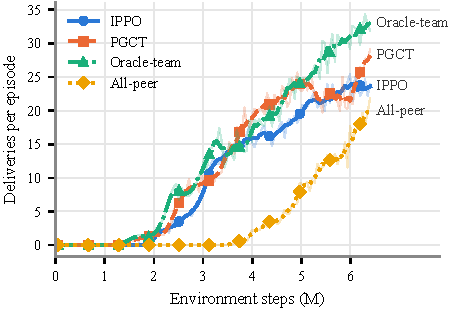
\includegraphics[width=\columnwidth]{figures/fig1_learning_curves.pdf}
\caption{E1의 평가 배송 수/episode(seed 1개\pilot). 가는 선: 51{,}200 step마다의 원 평가값, 굵은 선: 중심 5점 이동평균.}
\label{fig:curves}
\end{figure}

\textbf{학습.} 발견할 팀이 없어도 \ours{}는 모든 지표에서 독립 학습보다 나았다(표~\ref{tab:control}, 그림~\ref{fig:curves}).\pilot{} episode당 배송 1개에 0.26M step(13\%)
먼저 도달했고, 학습 중 평균 처리량은 12\%(11.7 대 10.4), 최종 처리량은 18\%(27.3 대 23.2) 높았다. episode당 배송 20개에 가장 먼저 도달했고(4.15M, Oracle-team 4.66M,
IPPO 5.07M), Oracle-team 평균 처리량의 89\%를 얻었다. 무차별 공유는 학습을 늦췄다. All-peer는 3.99M step에야 배송 1개에 도달했지만, 실행이 끝날 때 가장 빠르게 오르고 있었다.

\begin{figure*}[t]
\centering
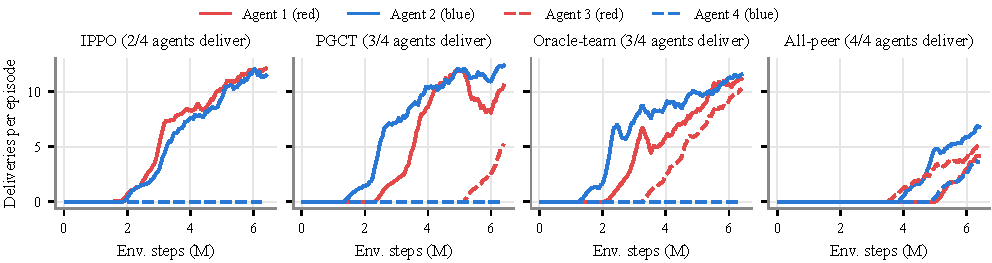
\includegraphics[width=\textwidth]{figures/fig2_per_agent_deliveries.pdf}
\caption{E1의 agent별 배송 수/episode(5점 이동평균, seed 1개\pilot). 빨강: 빨강 팀(agent 1, 3), 파랑: 파랑 팀(agent 2, 4). 실선: agent 1--2, 점선: agent 3--4.}
\label{fig:agents}
\end{figure*}

\textbf{뒤처진 agent.} agent별 곡선(그림~\ref{fig:agents})이 이득의 출처를 보여 준다. IPPO에서는 팀마다 한 명만 배송을 배웠다. 나머지 두 명은 계속 움직였지만 요청 선반을
한 번도 집지 않았다. 개인 보상이고 팀당 요청이 2개라, 먼저 배운 팀원이 요청 대부분을 처리하고 두 번째 팀원은 배울 만큼의 보상을 받지 못한다. critic distillation은 뒤처진
agent에게 자기 보상 없이도 가치 신호를 준다. \ours{}와 Oracle-team에서는 세 번째 agent가 배웠고(agent 3, 각각 5.4M과 3.6M step부터), All-peer에서는 늦었지만 네 명 모두
배웠다. 배운 agent 한 명이 episode당 약 10--12개를 배송하므로, 학습한 agent 수가 처리량 차이의 대부분을 설명한다. \todo{개입 실험: 뒤처진 agent의 distillation 차단;
seed별 학습 agent 수}

\begin{figure*}[t]
\centering
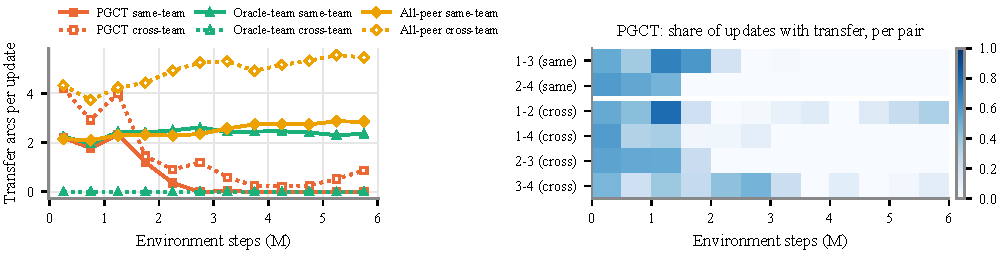
\includegraphics[width=\textwidth]{figures/fig3_critic_transfer.pdf}
\caption{E1의 실제 critic 전이(기록된 할당, warm-up 이후, seed 1개\pilot). 왼쪽: update당 방향성 전이 arc 수, 팀 안(실선)과 팀 간(점선), 0.5M step 구간 평균. 오른쪽:
\ours{}에서 각 agent 쌍이 critic 정보를 주고받은 update 비율.}
\label{fig:transfer}
\end{figure*}

\textbf{팀이 라벨로만 다를 때 \ours{}가 찾는 것.} 이 대조 조건에서 예상대로 probe 거리에는 팀 정보가 없었다. 2.5M step 이후 거의 모든 checkpoint와 모든 방법에서 팀원의
정책이 팀원이 아닌 쌍보다 \emph{덜} 비슷했다(그림~\ref{fig:jsgap}). 고정 모델에서도 팀을 가르도록 만든 집합을 포함한 probe 부분집합 5개 모두에서 같은 결과였다(부록 C).
팀 신호가 없자 추정 $\hat{\mathcal{T}}_i$는 역할과 숙련도를 따라갔다. 2M step 이후 팀을 가로질러 연결했고(agent 3--4, 이후 1--2; 4M step 이후 update당 같은 팀 0.03 arc,
다른 팀 0.63 arc, 그림~\ref{fig:transfer}), 연결된 쌍은 같은 역할(자기 구역에 머묾 / 상대 구역에서 선반을 가져옴)의 agent였다(부록 D). 이 대체 동작은 E1에서 해롭지 않았다.
별도의 고정 평가에서, receiver의 critic을 팀원의 critic과 섞었을 때의 가치 오차 감소가 팀원이 아닌 agent와 섞었을 때보다 \emph{작았다}(같은 팀 AUROC 0.25--0.33). 두 팀이
같은 과제를 풀기 때문이다. 또 \ours{}는 2M step 이후 baseline보다 훨씬 적게 전이했다(update의 37\%, 29\%; Oracle-team 82--86\%, All-peer 거의 100\%). 이 대조 조건은 두 가지를
보여 준다. 팀을 구분할 수 없을 때도 \ours{}는 해를 입지 않으며, 팀을 찾으려면 팀이 다르게 행동하는 환경이 필요하다.

\begin{figure}[t]
\centering
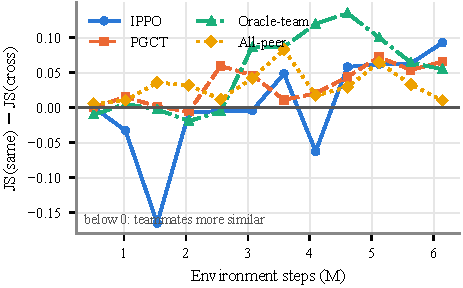
\includegraphics[width=\columnwidth]{figures/fig4_probe_js_gap.pdf}
\caption{E1 checkpoint에서 팀원 사이 probe 거리에서 팀원이 아닌 쌍의 probe 거리를 뺀 값(seed 1개\pilot). 0보다 크면 팀원의 정책이 더 다르다. 팀 대칭 대조 조건에는 팀 신호가 없다.}
\label{fig:jsgap}
\end{figure}

\section{목표가 분리된 팀(E1-F)}
\label{sec:main}
\todo{주 결과. E1-F 실행(IPPO, All-peer, Oracle-team, \ours{}, \ours{}-v2; 10M step; seed 1--$n$)이 끝나면 채운다.}
팀 발견 논리의 네 고리를 순서대로 평가한다.
(1) \emph{팀 단위 공유가 이로운가?} Oracle-team 대 All-peer.
(2) \emph{팀원의 critic이 더 호환되는가?} checkpoint에서 같은 팀과 다른 팀의 가치 호환성.
(3) \emph{\ours{}가 팀을 찾는가?} probe 거리 AUROC, 같은 팀 전이 비율, 행동 분화.
(4) \emph{팀 발견이 학습을 개선하는가?} \ours{}와 \ours{}-v2 대 IPPO, All-peer, Oracle-team.

\begin{table}[t]
\centering
\small
\resizebox{\columnwidth}{!}{%
\begin{tabular}{lccccc}
\toprule
방법 & 시작 & 평균 & 최종 & 같은 팀 전이 & Probe AUROC \\
\midrule
IPPO & \tbd & \tbd & \tbd & -- & \tbd \\
All-peer & \tbd & \tbd & \tbd & \tbd & \tbd \\
\ours{} & \tbd & \tbd & \tbd & \tbd & \tbd \\
\ours{}-v2 & \tbd & \tbd & \tbd & \tbd & \tbd \\
Oracle-team & \tbd & \tbd & \tbd & 100\% & \tbd \\
\bottomrule
\end{tabular}}
\caption{목표 분리 과제 E1-F. 같은 팀 전이: 실제 전이 arc 중 팀원 사이의 비율. Probe AUROC: checkpoint에서 probe 거리의 같은 팀 AUROC. \todo{실행이 끝나면 채움}}
\label{tab:main}
\end{table}

\begin{table}[t]
\centering
\small
\resizebox{\columnwidth}{!}{%
\begin{tabular}{lcccc}
\toprule
 & \multicolumn{2}{c}{E1 ($11\times10$)} & \multicolumn{2}{c}{E2 ($16\times16$)} \\
\cmidrule(lr){2-3}\cmidrule(lr){4-5}
방법 & AUC & 마지막 10회 & AUC & 마지막 10회 \\
\midrule
IPPO & 44.57 & 44.52 & 34.24 & 37.61 \\
\ours{} & 45.86 & 46.17 & 34.17 & 37.47 \\
\bottomrule
\end{tabular}}
\caption{보충: 팀 대칭 맵에서 공통 커리큘럼 checkpoint로부터 4M step 연장 학습(seed 1개\pilot; 학습률 $10^{-4}$, entropy 계수 0.02). 모든 agent가 이미 배송할 수 있으면
도울 뒤처진 agent가 없어 \ours{}의 이득이 작다.}
\label{tab:continuation}
\end{table}

\section{논의와 한계}
\textbf{팀 발견은 언제 중요한가?} 팀 발견이 도움이 되려면 팀이 다르게 행동해야 하고, 팀원의 가치 추정이 팀원이 아닌 agent의 것보다 서로에게 더 유용해야 한다. 팀 대칭 대조
조건은 둘 다 만족하지 않으며, 거기서 \ours{}는 호환성 기반 공유처럼 동작하면서도 뒤처진 agent를 도왔다. 목표 분리 과제에서 두 조건이 성립하는지, 그리고 그때 \ours{}가 팀을
찾는지가 핵심 실증 질문이다 \todo{E1-F}.

\textbf{예비 증거.} E1의 모든 수치는 training seed 1개에서 나왔다. 같은 seed와 가중치로 다시 실행하면 IPPO는 정확히 재현됐지만 공유 방식은 1.4--1.6M step 이후 갈라졌다(부록 B).
그 재실행에서 All-peer의 배송 시작은 2백만 step 차이가 났다. 그래서 여러 seed가 필요하며, 실행 중이다. \todo{평균과 95\% 구간; 비결정적 연산 확인}

\textbf{가정.} \ours{}는 공유 probe 집합, 모델 출력의 국소 통신, 같은 probe가 모든 agent에게 같은 상황을 뜻하는 관측을 가정한다. agent들이 팀 식별자를 직접 교환할 수도 있지만,
팀 발견은 목표가 비공개이거나, 조직 간에 라벨이 공유되지 않거나, 공통 어휘 없이 집단이 생길 때 의미가 있다. 우리 probe 집합은 맵 배치에서 고정 규칙으로 생성한다. 환경에 무관한
probe 생성은 향후 과제다.

\textbf{범위.} agent 4명, 팀 2개의 한 환경 계열이다. 더 많은 agent와 팀, 팀 공유 보상, 중앙 baseline(MAPPO, SePS 방식, HetDPS 방식)은 계획되어 있다. \todo{baseline}

\section{결론}
우리는 agent들이 공유 probe 집합에 대한 정책 응답으로 잠재 팀원을 발견하고 발견한 팀 안에서 critic을 공유하는 분산 방법 \ours{}를 제안했다. 행동으로 팀을 구분할 수 없는 팀 대칭
대조 조건에서 \ours{}는 비슷한 역할의 agent를 연결하는 쪽으로 물러났지만, 예비 실험에서 여전히 독립 학습과 무차별 공유를 앞섰다. 주로 뒤처진 agent가 학습하게 한 덕분이다. 목표
분리 과제는 \ours{}가 목표가 다른 팀을 찾아내는지, 그리고 그때 팀 단위 공유가 학습을 개선하는지를 보여 줄 것이다.

\bibliographystyle{plainnat}
\bibliography{references}

\clearpage
\appendix
\onecolumn

\section{하이퍼파라미터}
\begin{table}[h]
\centering
\small
\begin{tabular}{ll}
\toprule
Setting & Value \\
\midrule
Map / agents / teams & 11$\times$10 E1 / 4 / 2 \\
Reward & individual \\
Home-zone shelf ratio & 0.5 \\
Requests per team & 2 \\
Sensor / communication range & 5 / 5 \\
Learning rate & 0.0002 \\
Entropy coef. & 0.05 \\
$\gamma$ / GAE $\lambda$ & 0.99 / 0.95 \\
Rollout / BPTT length & 1024 / 64 \\
PPO epochs / minibatches / clip & 4 / 8 / 0.2 \\
Hidden (MLP / GRU) & 128 / 128 \\
Peer-loss coef. $\lambda_{peer}$ & 0.01 \\
Gate: JS threshold / EMA $\beta$ / warm-up & 0.12 / 0.35 / 100 upd. \\
Canonical probes & 48 (fixed, zero hidden, length 1) \\
Evaluation & every 50 updates, 20$\times$500 steps, deterministic \\
\bottomrule
\end{tabular}

\caption{처음부터 학습한 E1 비교의 설정(donor 집합을 제외하고 모든 방법이 동일).}
\end{table}

\section{같은 seed에서의 재현성}
\begin{figure}[h]
\centering
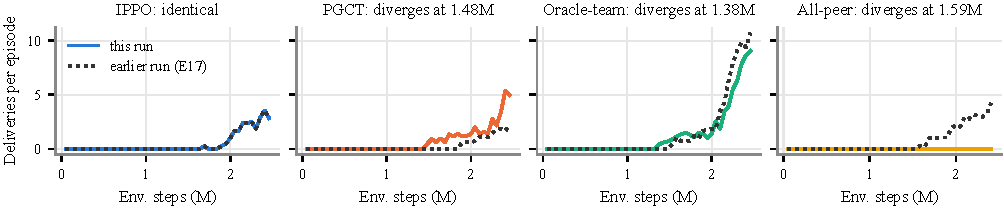
\includegraphics[width=\textwidth]{figures/figA1_reproducibility.pdf}
\caption{같은 seed와 초기 가중치의 두 실행(실선: 보고한 실행, 점선: 이전에 중단된 실행). IPPO는 정확히 재현되고, 공유 방식은 1.4--1.6M step 이후 갈라진다.}
\end{figure}

\section{고정 E1 모델에서의 probe 집합}
\begin{figure}[h]
\centering
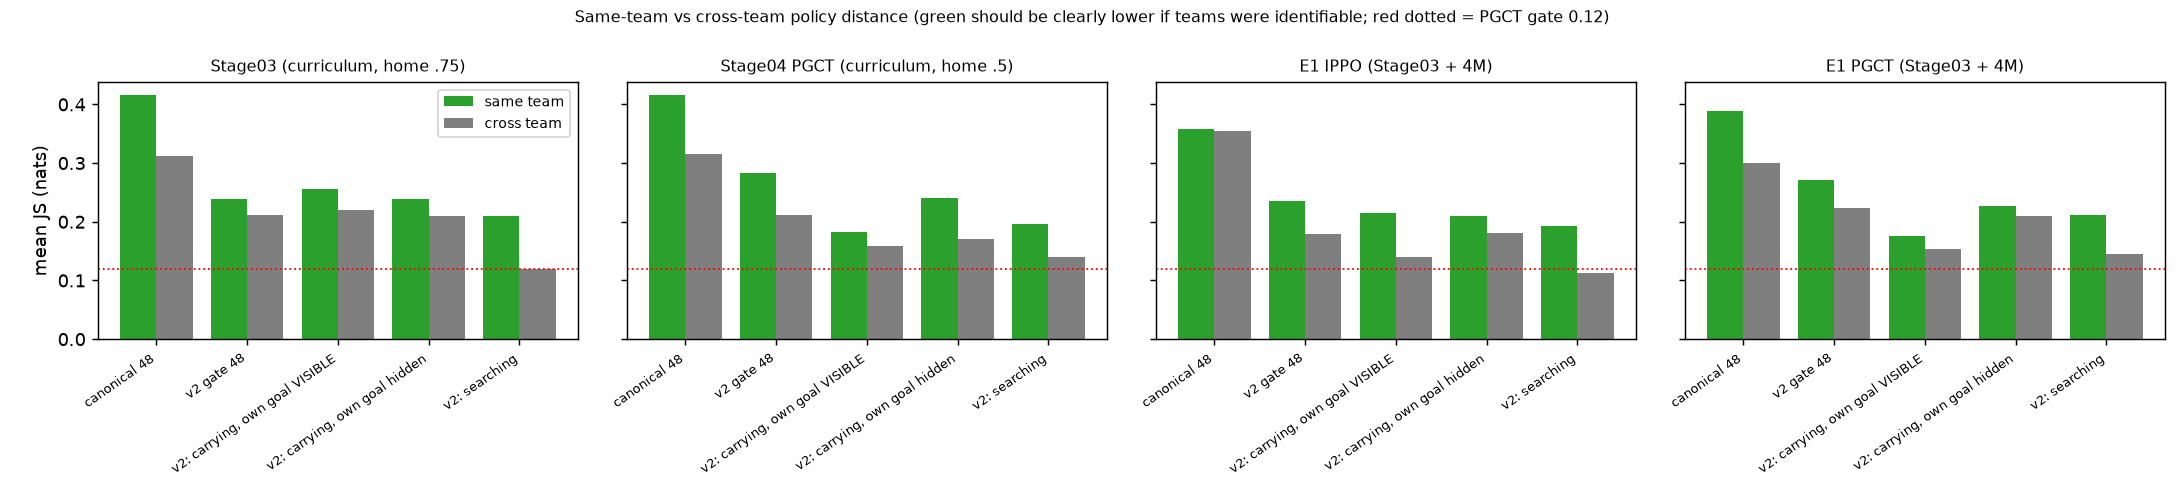
\includegraphics[width=\textwidth]{figures/frozen_probe_same_vs_cross.png}
\caption{고정 E1 모델 4개와 probe 부분집합 5개(팀을 가르도록 만든 ``적재 중, 목표 안 보임'' 집합 포함)에서 팀원(초록)과 팀원이 아닌 쌍(회색)의 평균 probe 거리. 팀 대칭
대조 조건에서는 20개 조합 모두 팀원이 덜 비슷하다. 빨간 점선: 임계값 0.12.}
\end{figure}

\section{커리큘럼 모델의 역할}
\begin{figure}[h]
\centering
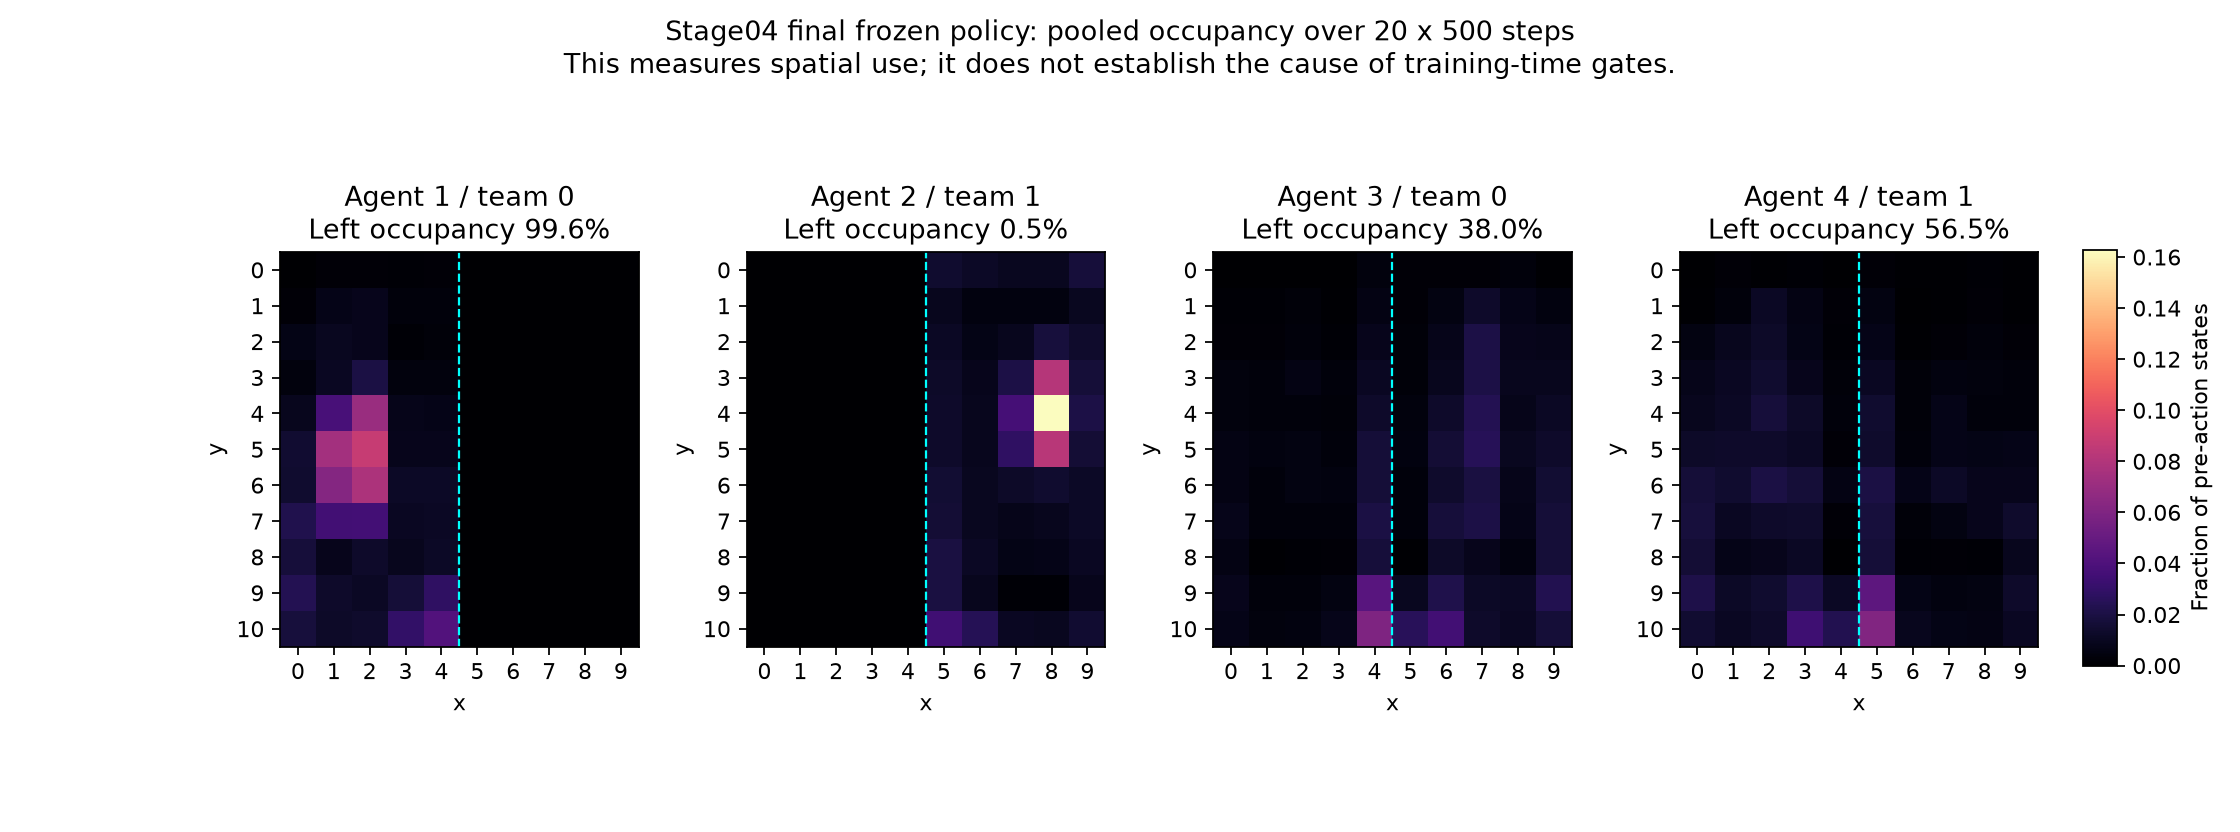
\includegraphics[width=\textwidth]{figures/stage04_occupancy.png}
\caption{선반의 50\%를 상대 팀 구역에 둔 고정 커리큘럼 모델의 칸 점유(20$\times$500 step). agent 1과 2는 자기 팀 구역에 머물고, agent 3과 4는 상대 구역에서 선반을 가져오며 gate가
가장 자주 연결한 쌍이다.}
\end{figure}

\section{구간별 실제 전이}
\begin{table}[h]
\centering
\small
\begin{tabular}{llccc}
\toprule
Method & Window & Updates w/ transfer & Same-team arcs/upd. & Cross-team arcs/upd. \\
\midrule
PGCT & 0--2.0M & 91\% & 1.86 & 3.09 \\
 & 2--4.0M & 37\% & 0.10 & 0.73 \\
 & 4--6.4M & 29\% & 0.03 & 0.63 \\
\addlinespace
Oracle-team & 0--2.0M & 82\% & 2.26 & 0.00 \\
 & 2--4.0M & 86\% & 2.50 & 0.00 \\
 & 4--6.4M & 85\% & 2.39 & 0.00 \\
\addlinespace
All-peer & 0--2.0M & 99\% & 2.22 & 4.18 \\
 & 2--4.0M & 100\% & 2.49 & 5.10 \\
 & 4--6.4M & 100\% & 2.79 & 5.37 \\
\bottomrule
\end{tabular}

\caption{E1의 학습 구간별 실제 전이(seed 1개). arc는 receiver--donor 방향 연결이다.}
\end{table}

\end{document}
